\section{Auswertung}
\label{sec:Auswertung}
\subsection{statistische Methode}
\begin{figure}[H]
  \centering
  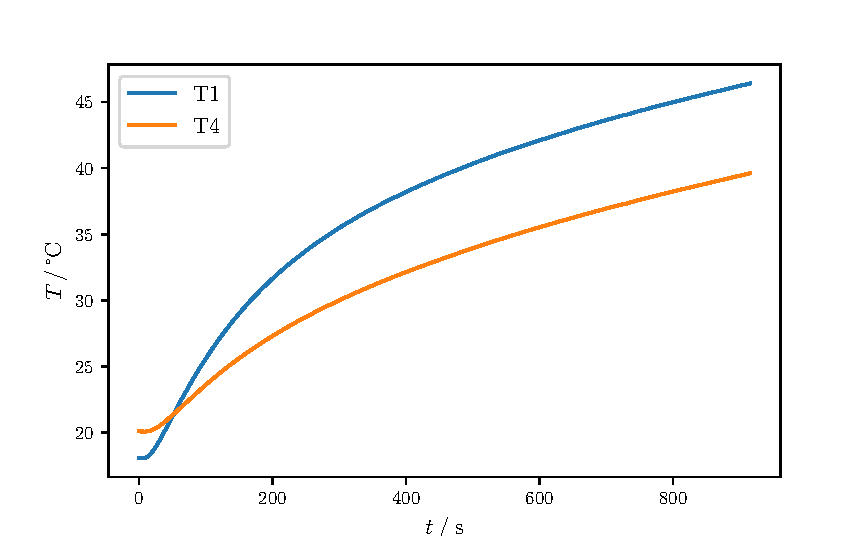
\includegraphics{plot1.pdf}
  \caption{Zeitlicher Temperaturverlauf des breiten und dünnen Messingstabes bei der statischen Methode}
  \label{fig:a}
\end{figure}

\begin{figure}[H]
  \centering
  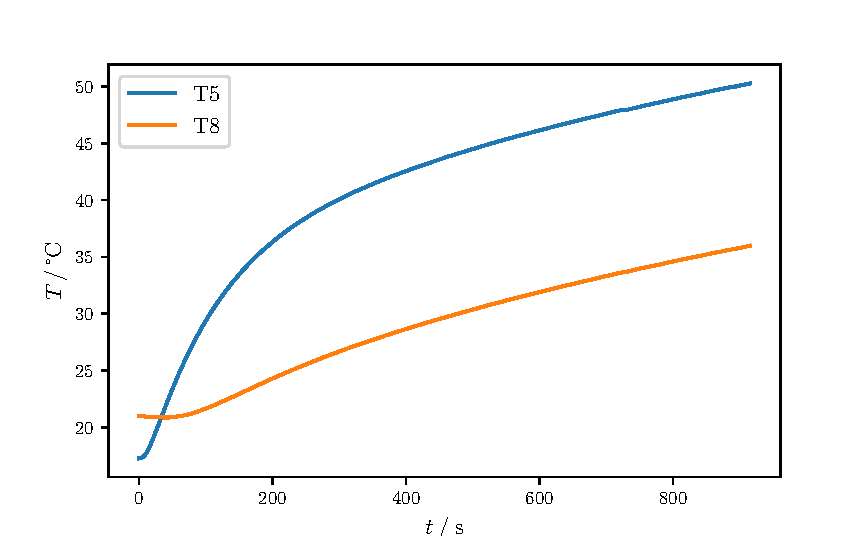
\includegraphics{plot2.pdf}
  \caption{Zeitlicher Temperaturverlauf des Aluminium- und Edelstahlstabes bei der statischen Methode}
  \label{fig:b}
\end{figure}

\noindent In Abbildung \ref{fig:a} sind die Temperaturverläufe der beiden Messingstäbe aufgetragen. Babei fällt auf, dass der breite Stab schneller
heißer wird als der dünne Stab und sich auf lange Sicht eine Temperaturdifferenz von ca $7\,\si{\celsius}$ einstellt. Auch wenn 
der dünne Messingstab zu Beginn der Messung eine höhere Starttemperatur von $20,1\,\si{\celsius}$ als der breite Messingstab ($18,07\,\si{\celsius}$) hatte, so wurde
diese Temperaturdifferenz bereits nach 45 Sekunden ausgeglichen.


\noindent In Abbildung \ref{fig:b} sind die Temperaturverläufe des Aluminiumstabes und des Edelstahlstabes aufgetragen. Hierbei
wird der Aluminiumstab schneller heiß als der Edelstahstab. Die Temperaturdifferenz stellt sich auf lange Sicht bei ca $14\,\si{\celsius}$ ein. Auch wenn 
der Edelstahstab zu Beginn der Messung eine höhere Starttemperatur von $21,01\,\si{\celsius}$ als der Aluminiumstab ($17,27\,\si{\celsius}$) hatte, so wurde
diese Temperaturdifferenz sogar schon nach nach 35 Sekunden ausgeglichen.


\noindent generell lässt sich sagen, dass alle Temperaturverläufe ihren größten Anstieg in den ersten 200 Sekunden haben. Dabei steigt die
Temperatur des Aluminiums schon nach den ersten Sekunden stark an, während Edelstahl sich erst nach einer Minute merkbar erwärmt.
Um beurteilen zu können, welcher Stab die beste Wärmeleitung hat, werden die Temperaturen nach 700 Sekunden verglichen (Siehe Tabelle \ref{tab:a}).

\begin{table}
\centering
\caption{Temperatur der Thermoelemente nach 700 Sekunden}
\label{tab:a}
\sisetup{table-format=1.2}
\begin{tabular}{S[table-format=3.0] S S[table-format=3.2]}
\toprule
{Thermoelement} & {$T\,/\,\si{\celsius}$}\\
\midrule
T1 & 43,62\\
T4 & 36,94\\
T5 & 47,62\\
T8 & 33,32\\

\bottomrule
\end{tabular}
\end{table}

\noindent Es lässt sich also sagen, dass der Aluminiumstab die beste Wärmeleitung hat.\\


\noindent In den Abbildungen \ref{fig:c} und \ref{fig:d} sind die Temperaturdifferenzen des nahen und fernen Thermoelementes des breiten
Messingstabes und des Edelstahlstabes gegen die Zeit aufgetragen.
\begin{figure}[H]
  \centering
  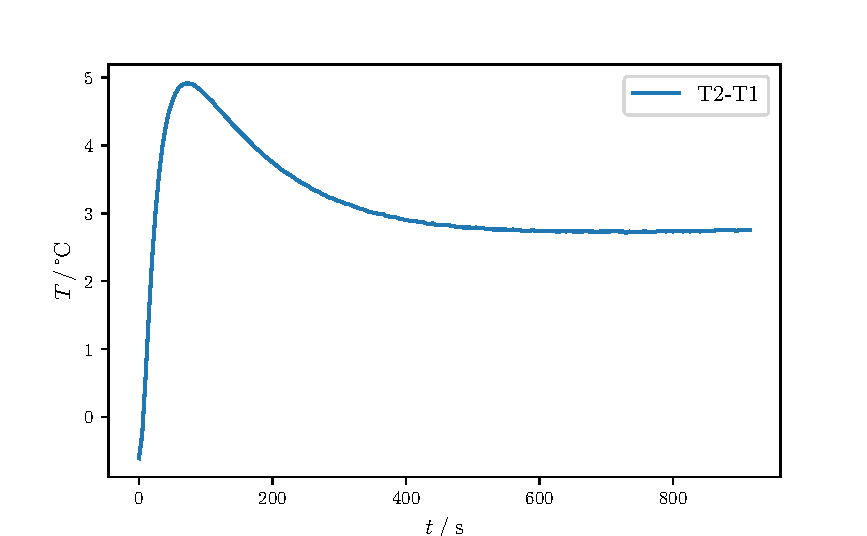
\includegraphics{diff1.pdf}
  \caption{Zeitlicher Verlauf der Temperaturdifferenz zwischen T1 und T2 am Messingstab bei der statischen Methode}
  \label{fig:c}
\end{figure}

\begin{figure}[H]
  \centering
  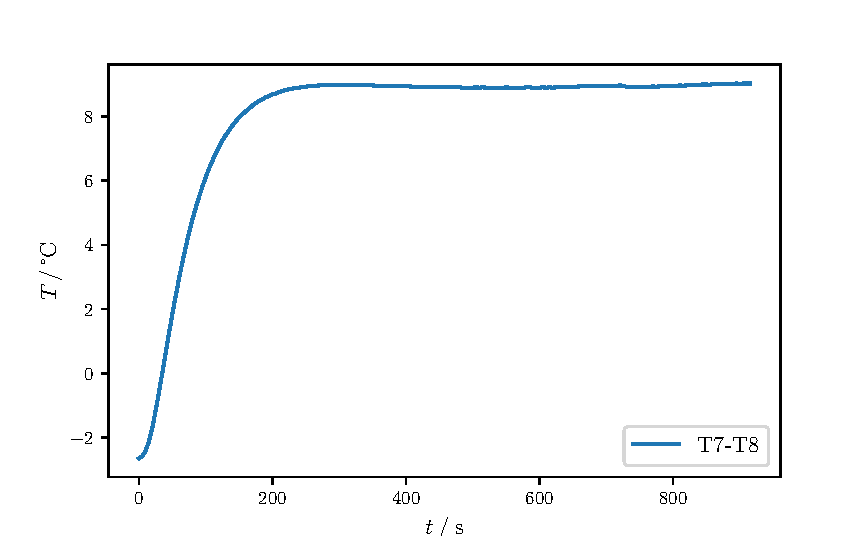
\includegraphics{diff2.pdf}
  \caption{Zeitlicher Verlauf der Temperaturdifferenz zwischen T7 und T8 am Edelstahstab bei der statischen Methode}
  \label{fig:d}
\end{figure}

\noindent Beide Verläufe nähern sich nach einiger Zeit einem festen Wert an. Die Temperaturdifferenz beim Messingstab
stellt sich nach ca 400 Sekunden auf  $2,8\,\si{\celsius}$ ein und die des Edelstabstabes nach schon 200 Sekunden auf $9,5\si{\celsius}$.
Der größte Unterschied zwischen den beiden Graphen ist der, dass die Temperaturdifferenz des Messingstabes zunächst auf $5\,\si{\celsius}$ ansteigt, bevor sich der
gleichbleibende Wert einspielt. Beim Messingstab nähert sich der Graph von unten seiner oberen Schranke an und überschreitet diese nicht.


\subsection{Dynamische Methode}
\begin{figure}[H]
  \centering
  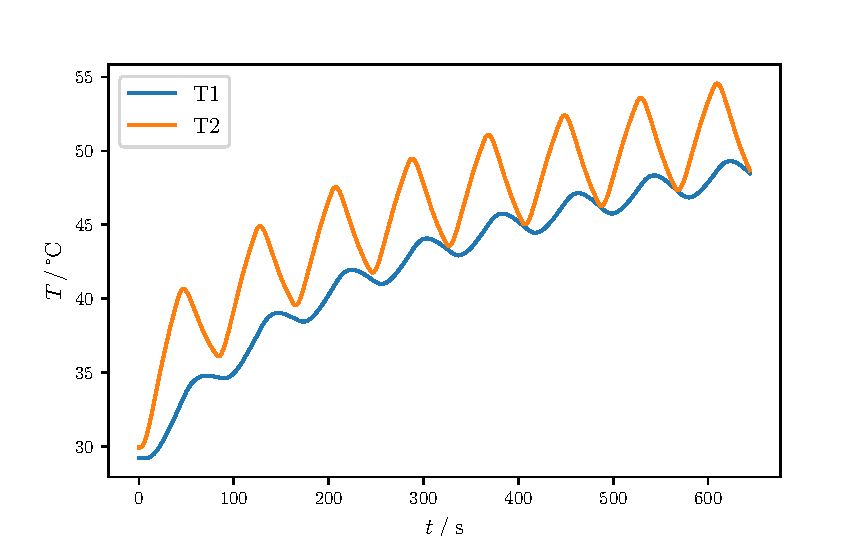
\includegraphics{plot3.pdf}
  \caption{Zeitlicher Temperaturverlauf von T1 und T2 am Messingstab bei der dynamischen Methode}
  \label{fig:e}
\end{figure}


\begin{figure}[H]
  \centering
  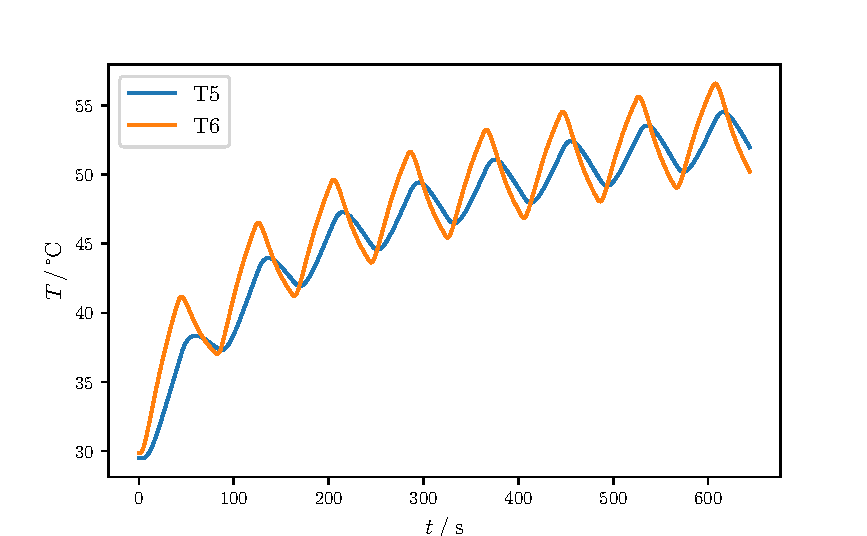
\includegraphics{plot4.pdf}
  \caption{Zeitlicher Temperaturverlauf von T7 und T8 am Edelstahlstabes bei der dynamischen Methode}
  \label{fig:f}
\end{figure}

